\documentclass[aspectratio=169, 14pt]{beamer}
\usepackage[utf8]{inputenc}
\usepackage[english]{babel}
\usepackage{tipa}
\usepackage{graphicx}
\usepackage{transparent}
\usepackage[ruled, lined, linesnumbered, commentsnumbered]{algorithm2e}
\newcommand\mycommfont[1]{\small\ttfamily\textcolor{blue}{#1}}
\SetCommentSty{mycommfont}
\renewcommand{\thealgocf}{}
\usepackage{setspace}
\usepackage{pgfplots}
\usepackage{tikz}
\usetikzlibrary{matrix,backgrounds}
\usetikzlibrary{arrows}
\usetikzlibrary {arrows.meta}
\usetikzlibrary{calc,shadows.blur,fit,positioning}
\usetikzlibrary{shapes.multipart,chains}
\usepackage{minted}
\usepackage{fontawesome5}
\usepackage{booktabs}
\usepackage{caption}
\usepackage{hyperref}
\hypersetup{
	colorlinks=true,
	linkcolor=blue,
	filecolor=magenta,
	urlcolor=cyan,
}
\urlstyle{same}
\usetheme{metropolis}
\metroset{block=fill}
\usecolortheme{default}
\definecolor{darkmidnightblue}{rgb}{0.0, 0.2, 0.4}
\definecolor{LightGray}{gray}{0.9}


%------------------------------------------------------------
%This block of code defines the information to appear in the
%Title page
\title[Data Structures] %optional
{Data Structures}

\subtitle{Linked Lists}

\author[CHEN Zhongpu] % (optional)
{CHEN Zhongpu}

\institute[] % (optional)
{
	School of Computing and Artificial Intelligence \\
	\href{mailto:zpchen@swufe.edu.cn}{zpchen@swufe.edu.cn}
}

\date[] % (optional)
{SWUFE, Fall \the\year{}}

%End of title page configuration block
%------------------------------------------------------------


%------------------------------------------------------------
%The next block of commands puts the table of contents at the 
%beginning of each section and highlights the current section:

% \AtBeginSection[]
% {
%   \begin{frame}
%     \frametitle{Table of Contents}
%     \tableofcontents[currentsection]
%   \end{frame}
% }
%------------------------------------------------------------


\begin{document}

%The next statement creates the title page.
\frame{\titlepage}

%---------------------------------------------------------
%This block of code is for the table of contents after
%the title page
% \begin{frame}
% \frametitle{Table of Contents}
% \tableofcontents
% \end{frame}
%--------------------------------------------------------
\begin{frame}
	\frametitle{A Small Quiz}
	\begin{enumerate}
		\item A queue implements a LIFO policy. (True or False)
		\item What does \texttt{[None] * 10} mean in Python?
		\item What is a \texttt{deque}?
	\end{enumerate}
\end{frame}

{
% \usebackgroundtemplate{\transparent{0.3}{\begin{picture}
%     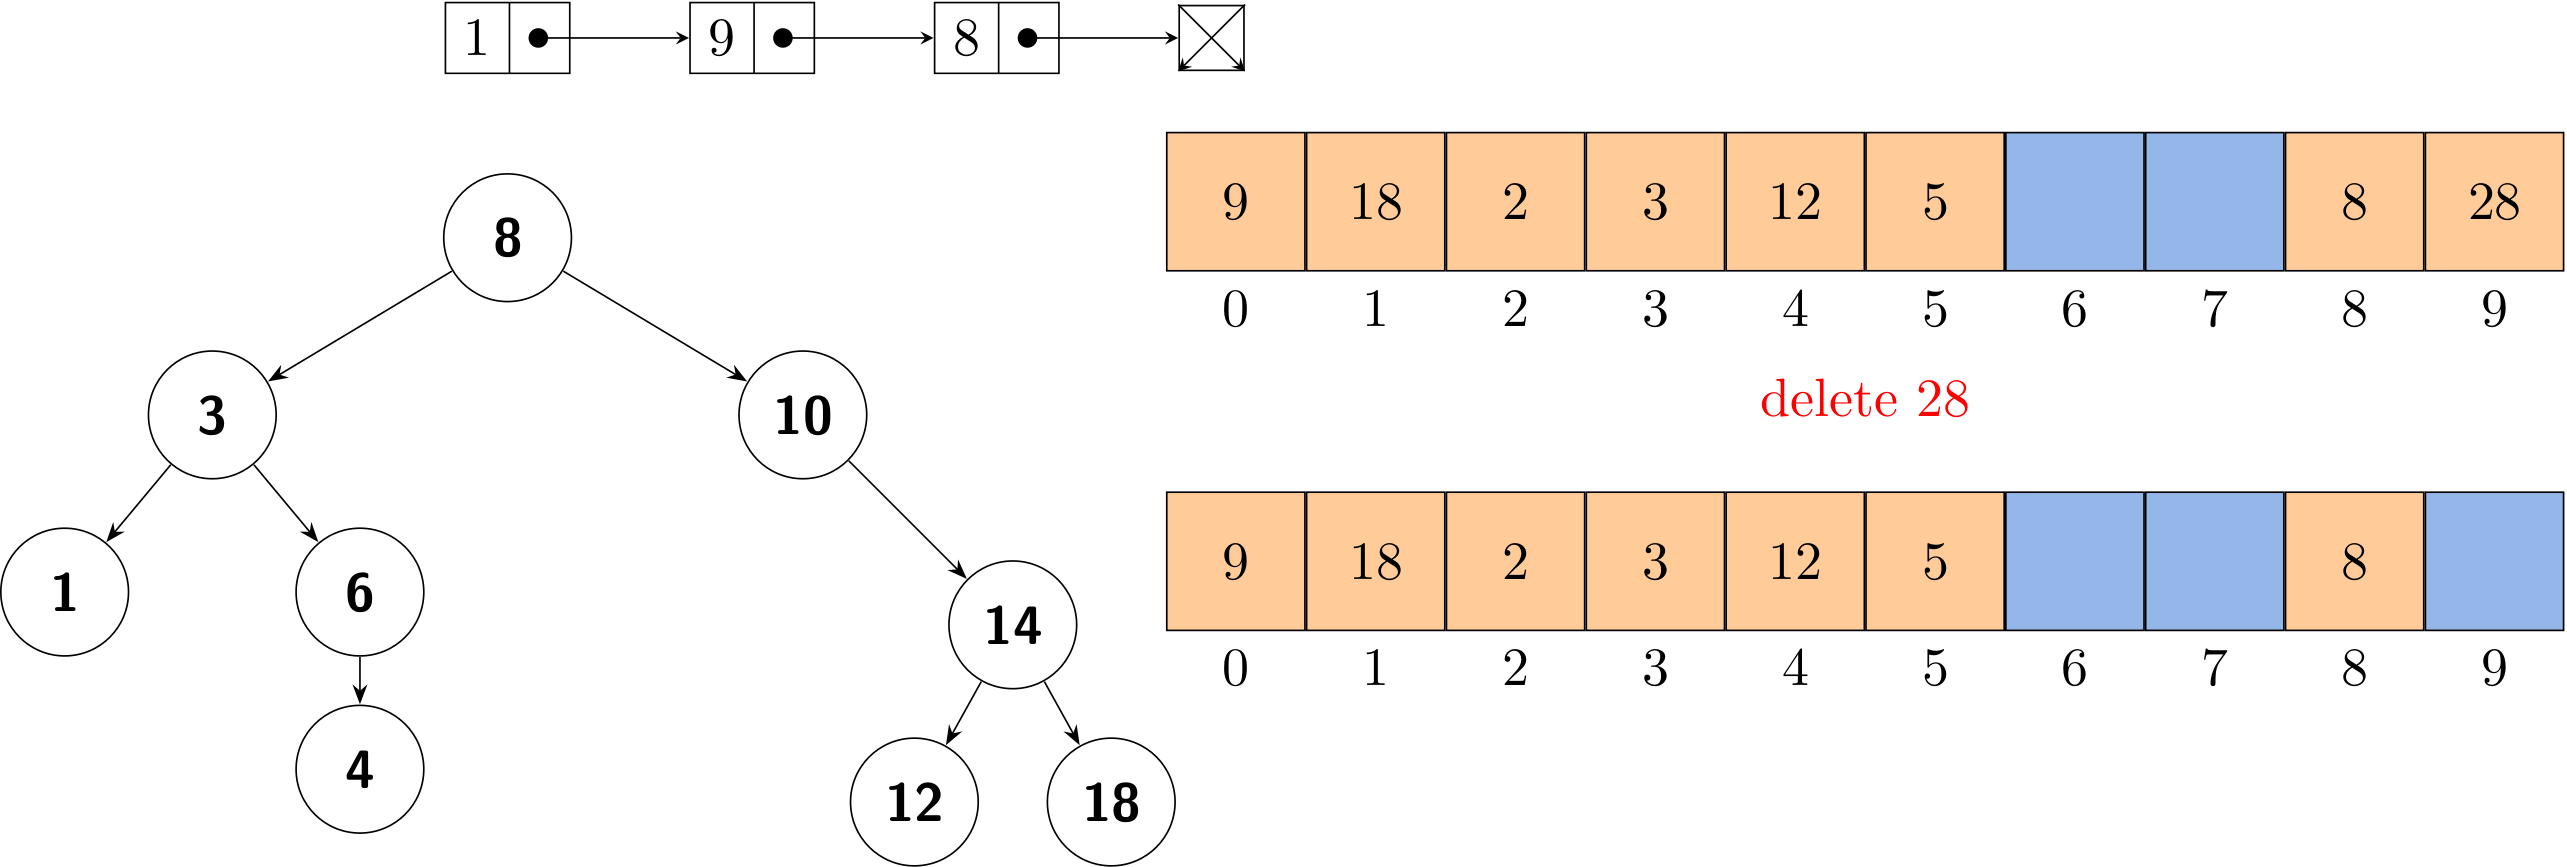
\includegraphics[height=0.7\paperheight]{cover}
% \end{picture}    
% }}
\usebackgroundtemplate{
	\tikz[overlay,remember picture]
	\node[opacity=0.3, at=(current page.south east),anchor=south east, yshift=2cm,xshift=4cm] {
		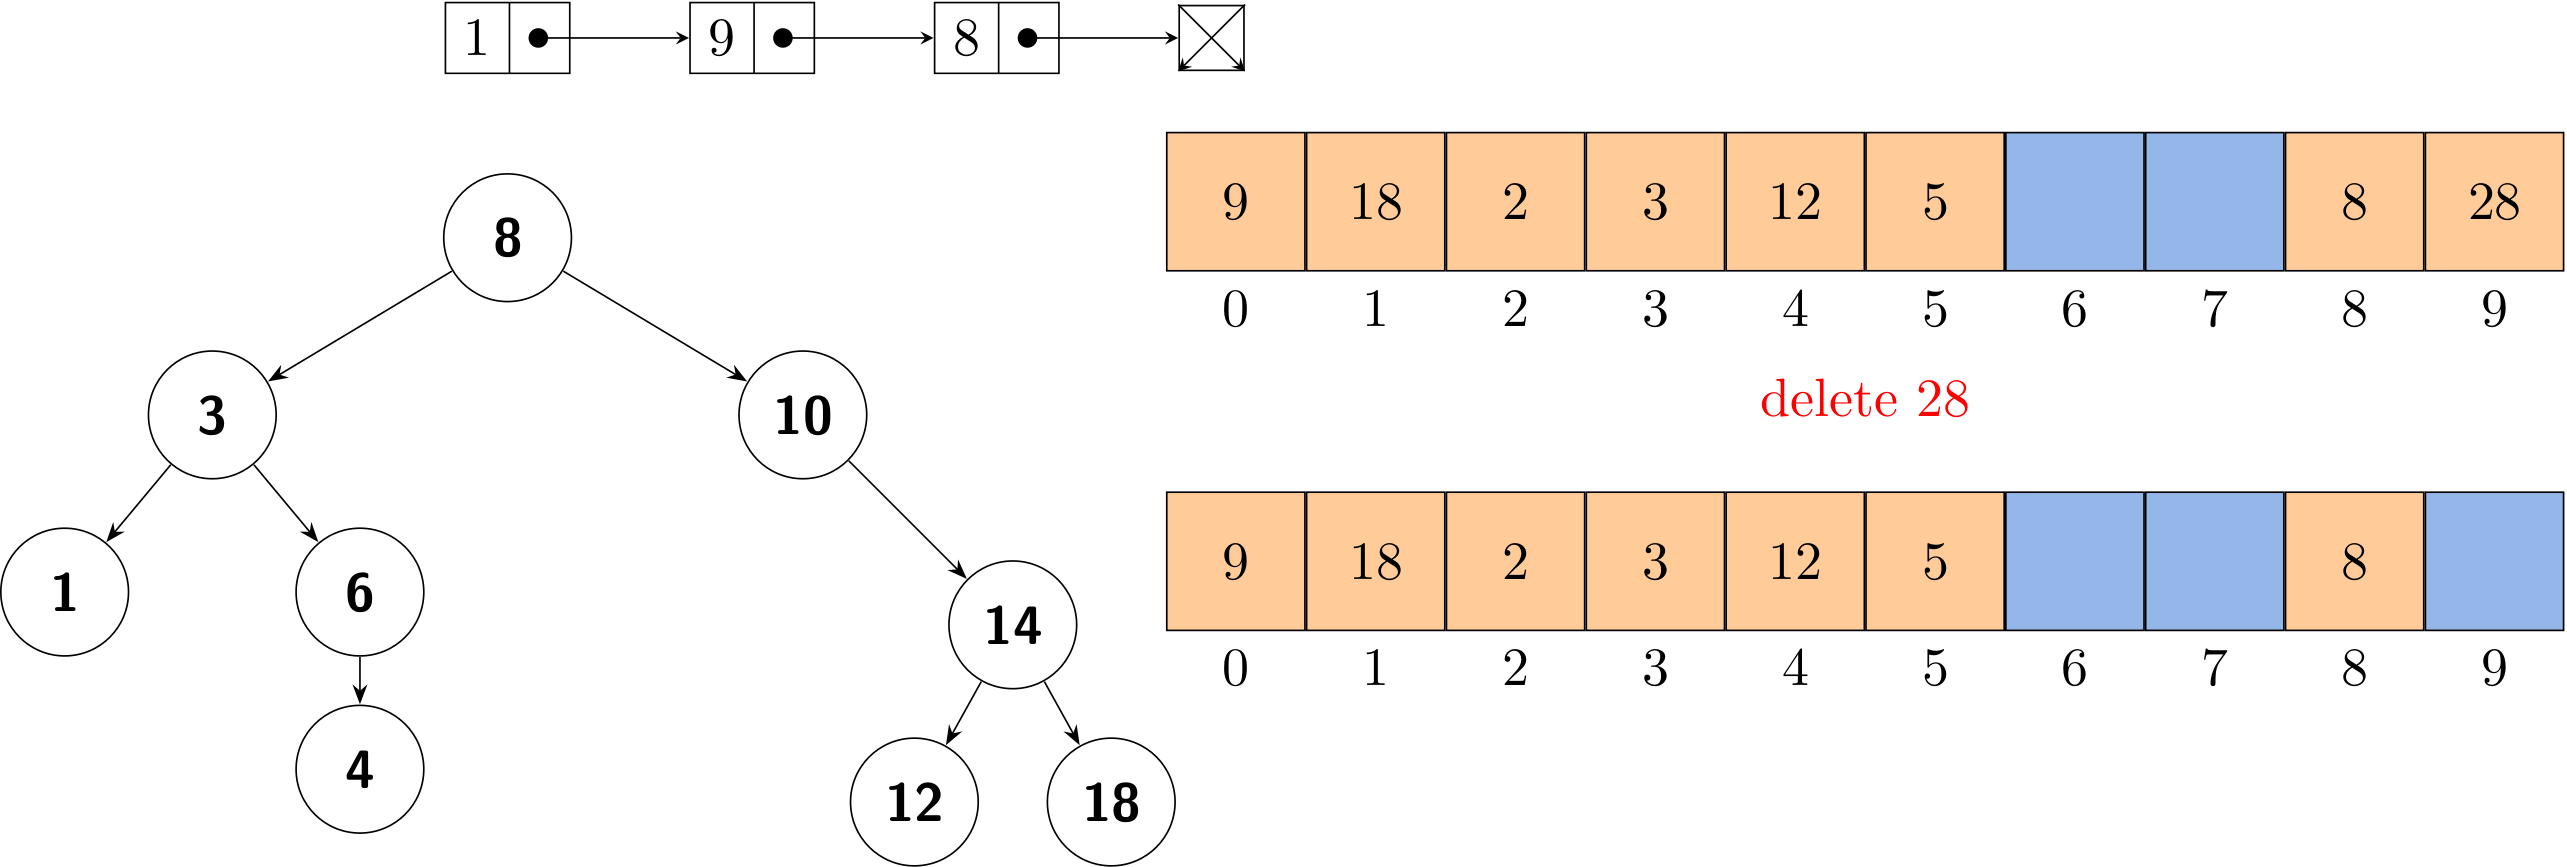
\includegraphics[height=0.6\paperheight]{cover}};
}
\begin{frame}
	\section{\textcolor{darkmidnightblue}{1. List ADT}}
\end{frame}

}

\begin{frame}

	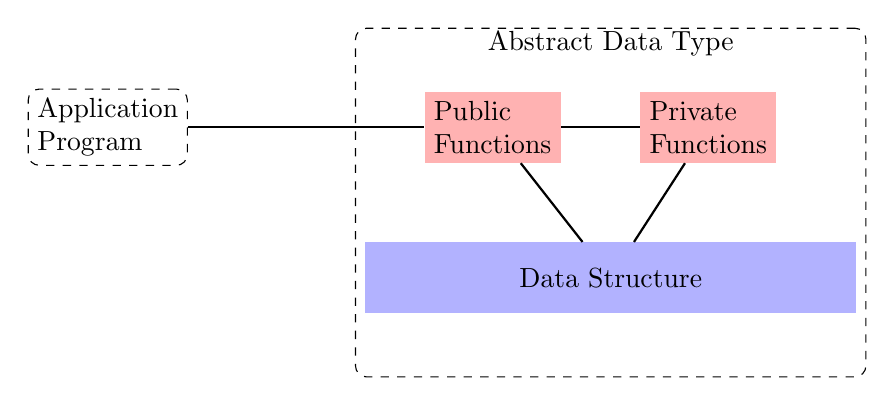
\begin{tikzpicture}[slot/.style={minimum size=0.9cm,rectangle}, data/.style={slot, fill=black!30},
			data2/.style={slot, fill=red!30},data3/.style={slot, fill=blue!30, align=center, text width=6cm}, >=Stealth]

		\node[draw, rounded corners, dashed, align=left](app){Application\\Program};

		\node[data2, align=left, right=of app, xshift=2cm] (public){Public\\Functions};
		\node[data2, align=left, right=of public](private){Private\\Functions};
		\node[data3, below=of public, xshift=1.5cm](data){Data Structure};

		\node [draw, rounded corners, inner ysep=.8cm, dashed,
			fit=(public) (private) (data), label={[anchor=north, inner sep=1pt]north:Abstract Data Type}]{};

		\draw[thick] (app) -- (public);
		\draw[thick] (public) -- (private);
		\draw[thick] (public) -- (data);
		\draw[thick] (private) -- (data);

	\end{tikzpicture}


	\begin{quote}
		An abstract data type (\alert{ADT}) is a class (or type) of objects whose logical behavior is defined by a set of values and \underline{a set of operations}.
	\end{quote}

\end{frame}
\begin{frame}
	\frametitle{1.1 List}

	\begin{exampleblock}{List}
		An ordered collection (also known as a sequence).
	\end{exampleblock}

	\begin{itemize}
		\item \texttt{add(e)}
		\item \texttt{get(i)}
		\item \texttt{remove(i)}
		\item \texttt{size()}
		\item ...
	\end{itemize}
	For users, they only care about what operations can be performed, but not \textbf{how these operations will be implemented}.

\end{frame}


\begin{frame}[fragile]
	\frametitle{1.2 Revisit List}
	\texttt{ArrayList} in Java and \texttt{list} in Python are both based on \textbf{arrays}. Therefore, the elements are occupying \textbf{contiguous} memories.

	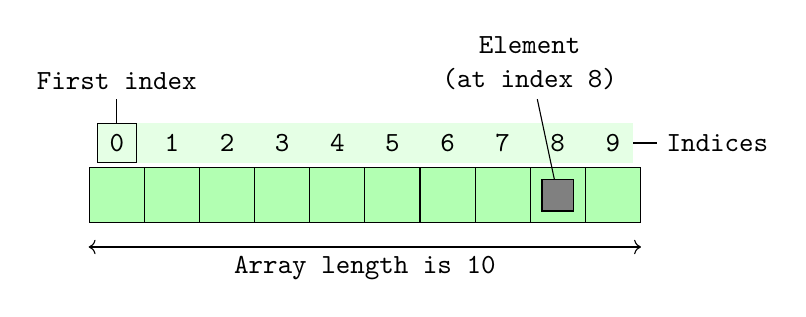
\begin{tikzpicture}[font=\ttfamily,
			array/.style={matrix of nodes,nodes={draw, minimum size=7mm, fill=green!30},column sep=-\pgflinewidth, row sep=0.5mm, nodes in empty cells,
					row 1/.style={nodes={draw=none, fill=none, minimum size=5mm}},
					row 1 column 1/.style={nodes={draw}}}]

		\matrix[array] (array) {
			0 & 1 & 2 & 3 & 4 & 5 & 6 & 7 & 8 & 9                        \\
			  &   &   &   &   &   &   &   &   & \\};
		\node[draw, fill=gray, minimum size=4mm] at (array-2-9) (box) {};

		\begin{scope}[on background layer]
			\fill[green!10] (array-1-1.north west) rectangle (array-1-10.south east);
		\end{scope}

		\draw[<->]([yshift=-3mm]array-2-1.south west) -- node[below] {Array length is 10} ([yshift=-3mm]array-2-10.south east);

		\draw (array-1-1.north)--++(90:3mm) node [above] (first) {First index};
		\draw (array-1-10.east)--++(0:3mm) node [right]{Indices};
		\node [align=center, anchor=south] at (array-2-9.north west|-first.south) (8) {Element\\ (at index 8)};
		\draw (8)--(box);
	\end{tikzpicture}


\end{frame}

\begin{frame}[fragile]

	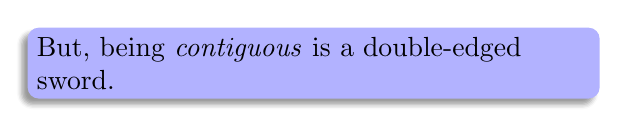
\begin{tikzpicture}
		\node[fill=blue!30,blur shadow={shadow xshift=-0.5ex},
			text width=20em,anchor=south west,rounded corners]
		{But, being \emph{contiguous} is a double-edged sword.};
	\end{tikzpicture}

	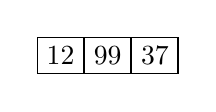
\begin{tikzpicture}
		\matrix[nodes=draw]
		{
			\node {12}; &
			\node {99}; &
			\node {37};   \\
		};
	\end{tikzpicture}

	\begin{itemize}
		\item Efficient in many index-based operations (e.g., \texttt{get(i)}).
		\item Inefficient while shifting or copying (e.g., removing the 1st element).
	\end{itemize}

	\pause

	As for the List ADT, there is yet another implementation, named \alert{linked lists}, which are not \emph{contiguous} in the memory.

	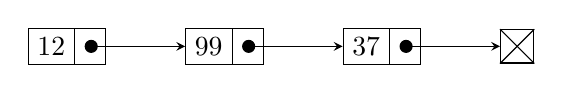
\begin{tikzpicture}[list/.style={rectangle split, rectangle split parts=2,
					draw, rectangle split horizontal}, >=stealth, start chain]

		\node[list,on chain] (A) {12};
		\node[list,on chain] (B) {99};
		\node[list,on chain] (C) {37};
		\node[on chain,draw,inner sep=6pt] (D) {};
		\draw (D.north east) -- (D.south west);
		\draw (D.north west) -- (D.south east);
		\draw[*->] let \p1 = (A.two), \p2 = (A.center) in (\x1,\y2) -- (B);
		\draw[*->] let \p1 = (B.two), \p2 = (B.center) in (\x1,\y2) -- (C);
		\draw[*->] let \p1 = (C.two), \p2 = (C.center) in (\x1,\y2) -- (D);
	\end{tikzpicture}

\end{frame}

\begin{frame}

	\section{\textcolor{darkmidnightblue}{2. Linked Lists}}

	\begin{quote}
		A linked list is a data structure in which the objects are arranged in a linear order, and the order in a linked list is determined by a pointer in each object.
	\end{quote}

\end{frame}

\begin{frame}
	\frametitle{2.1 Definition}

	\begin{columns}
		\column{.5\textwidth}
		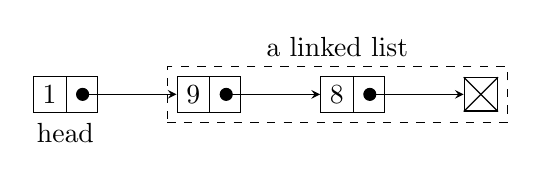
\begin{tikzpicture}[list/.style={rectangle split, rectangle split parts=2,
						draw, rectangle split horizontal}, >=stealth, start chain]

			\node[list,on chain] (A) {1};
			\node[list,on chain] (B) {9};
			\node[list,on chain] (C) {8};
			\node[on chain,draw,inner sep=6pt] (D) {};
			\draw (D.north east) -- (D.south west);
			\draw (D.north west) -- (D.south east);
			\draw[*->] let \p1 = (A.two), \p2 = (A.center) in (\x1,\y2) -- (B);
			\draw[*->] let \p1 = (B.two), \p2 = (B.center) in (\x1,\y2) -- (C);
			\draw[*->] let \p1 = (C.two), \p2 = (C.center) in (\x1,\y2) -- (D);
			\node[below=of A, yshift=1cm] (head){\alert{head}};

			\node[fit=(B)(C)(D), dashed, draw](remain) {};

			\node[above=of remain, yshift=-1cm]{\alert{a linked list}};

		\end{tikzpicture}
		\column{.4\textwidth}
		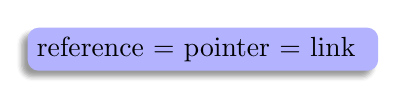
\begin{tikzpicture}
			\node[fill=blue!30,blur shadow={shadow xshift=-0.5ex},
				text width=12em,anchor=south west,rounded corners]
			{reference = pointer = link};
		\end{tikzpicture}
	\end{columns}

	\begin{quote}
		A linked list is a \textbf{recursive} data structure that is either empty (null) or a reference to a node having an item and a reference to a linked list.
	\end{quote}

	
\begin{tikzpicture}
		\node[fill=yellow,blur shadow={shadow xshift=-0.5ex},
			text width=25em,anchor=south west,rounded corners]
		{We can use the \alert{\texttt{head}} node to represent a linked list.};
	\end{tikzpicture}

\end{frame}

\begin{frame}[fragile]
	\frametitle{Node}
	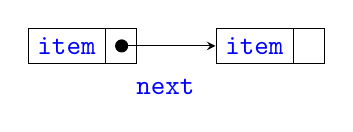
\begin{tikzpicture}[list/.style={rectangle split, rectangle split parts=2,
					draw, rectangle split horizontal}, >=stealth, start chain]

		\node[list,on chain] (A) {\textcolor{blue}{\texttt{item}}};
		\node[list,on chain] (B) {\textcolor{blue}{\texttt{item}}};

		\draw[*->] let \p1 = (A.two), \p2 = (A.center) in (\x1,\y2) -- node[below, yshift=-.3cm] {\textcolor{blue}{\texttt{next}}}(B);
	\end{tikzpicture}

	\begin{minted}[bgcolor=LightGray, baselinestretch=1]{python}
class Node:
    def __init__(self, item, next=None):
        self.item = item
        self.next = next

class LinkedList:
    def __init__(self, head=None):
        self.head = head
    \end{minted}
\end{frame}


\begin{frame}
	\frametitle{2.2 Pseudo-code}

	\begin{quote}
		The term \alert{pseudo-code} refers to an informal, English-like notation for describing how an algorithm, a method, a class, or a program will work.
	\end{quote}

	\begin{exampleblock}{Example}
		\texttt{indexOf(a, o)} which returns the index of the first occurrence of the specified element \texttt{o} in array \texttt{a}, or -1 if \texttt{a} does not contain \texttt{o}.
	\end{exampleblock}
\end{frame}

\begin{frame}[fragile]

	\begin{exampleblock}{Example}
		\texttt{indexOf(a, o)} which returns the index of the first occurrence of the specified element \texttt{o} in array \texttt{a}, or -1 if \texttt{a} does not contain \texttt{o}.
	\end{exampleblock}

	\scalebox{.8}{
		\begin{algorithm}[H]
			\caption{indexOf(a, o)}
			$n\gets a.size()$ \\
			\For{$i\gets 0$ \KwTo $n$}{
				\If{$a[i] == o$}{
					\Return{i}
				}
			}
			\Return{-1}
		\end{algorithm}
	}
	\pause
	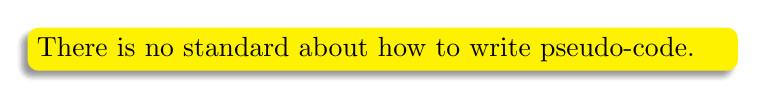
\begin{tikzpicture}
		\node[fill=yellow,blur shadow={shadow xshift=-0.5ex},
			text width=25em,anchor=south west,rounded corners]
		{There is no standard about how to write pseudo-code.};
	\end{tikzpicture}
\end{frame}

\begin{frame}
	\frametitle{Exercise}
	{\large \faIcon{code}} Given the \alert{\texttt{head}} of a linked list, how to check whether it is empty or not?

	\pause

	\scalebox{.8}{
		\begin{algorithm}[H]
			\caption{isEmpty(head)}
			\KwIn{Head node $head$ of a linked list.}
			\KwOut{Return true if it is empty.}
			\Return{head == null}
		\end{algorithm}
	}

	{\large \faIcon{code}} Given the \alert{\texttt{head}} of a linked list, how to check whether its size is one?
\end{frame}

{\setbeamercolor{palette primary}{fg=black, bg=yellow}
\begin{frame}[standout]
	In what follows, I will describe the algorithms using pseudo-code.
\end{frame}
}

\begin{frame}
	\frametitle{2.3 Common Operations: search()}
	Given the \alert{\texttt{head}} of a linked list, find the first element with item \alert{\texttt{k}} in this list, returning a pointer to this element.

	\scalebox{.8}{
		\begin{algorithm}[H]
			\caption{search(head, k)}
			\KwIn{The $head$ of a linked list, and a target $k$.}
			\KwOut{Return the node whose item is $k$.}
			$x\gets head$ \\
			\While{x $\neq$ null and x.item $\neq$ k} {
				$x\gets x.next$
			}
			\Return{x}
		\end{algorithm}
	}

	{\large \faIcon{question-circle}} \textbf{Question}: What is the time complexity of \texttt{search()}?
\end{frame}

\begin{frame}
	\frametitle{Exercise 1}
	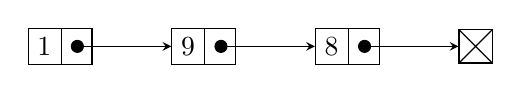
\begin{tikzpicture}[list/.style={rectangle split, rectangle split parts=2,
					draw, rectangle split horizontal}, >=stealth, start chain]

		\node[list,on chain] (A) {1};
		\node[list,on chain] (B) {9};
		\node[list,on chain] (C) {8};
		\node[on chain,draw,inner sep=6pt] (D) {};
		\draw (D.north east) -- (D.south west);
		\draw (D.north west) -- (D.south east);
		\draw[*->] let \p1 = (A.two), \p2 = (A.center) in (\x1,\y2) -- (B);
		\draw[*->] let \p1 = (B.two), \p2 = (B.center) in (\x1,\y2) -- (C);
		\draw[*->] let \p1 = (C.two), \p2 = (C.center) in (\x1,\y2) -- (D);

	\end{tikzpicture}

	{\large \faIcon{code}} How to implement \texttt{contains(head, k)} based on \texttt{search(head, k)}?

	\begin{itemize}
		\item \texttt{contains(head, 9)} returns \texttt{true}.
		\item \texttt{contains(head, 6)} returns \texttt{false}.
	\end{itemize}

\end{frame}

\begin{frame}[fragile]
	\frametitle{Exercise 2}
	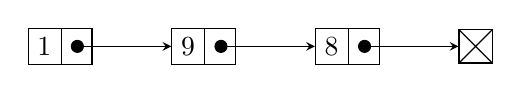
\begin{tikzpicture}[list/.style={rectangle split, rectangle split parts=2,
					draw, rectangle split horizontal}, >=stealth, start chain]

		\node[list,on chain] (A) {1};
		\node[list,on chain] (B) {9};
		\node[list,on chain] (C) {8};
		\node[on chain,draw,inner sep=6pt] (D) {};
		\draw (D.north east) -- (D.south west);
		\draw (D.north west) -- (D.south east);
		\draw[*->] let \p1 = (A.two), \p2 = (A.center) in (\x1,\y2) -- (B);
		\draw[*->] let \p1 = (B.two), \p2 = (B.center) in (\x1,\y2) -- (C);
		\draw[*->] let \p1 = (C.two), \p2 = (C.center) in (\x1,\y2) -- (D);

	\end{tikzpicture}

	{\large \faIcon{code}} Given the \alert{\texttt{head}} of a linked list, how to return the size of the list?

	\pause

	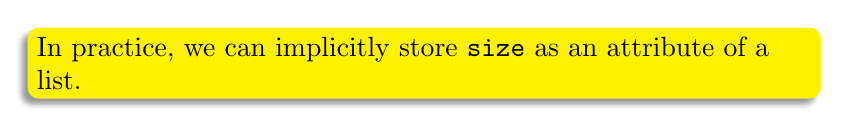
\begin{tikzpicture}
		\node[fill=yellow,blur shadow={shadow xshift=-0.5ex},
			text width=28em,anchor=south west,rounded corners]
		{In practice, we can implicitly store \texttt{size} as an attribute of a list.};
	\end{tikzpicture}

	\begin{minted}[bgcolor=LightGray, baselinestretch=1]{python}
class LinkedList:
    def __init__(self):
        self.head = None
        self.size = 0
\end{minted}

\end{frame}

\begin{frame}
	\frametitle{2.3 Common Operations: addFirst()}

	To add an element at the beginning of the list. The core idea is to \textbf{create a new node whose \texttt{next} is the current \texttt{head}, and then update \texttt{head} to this newly created node}.

	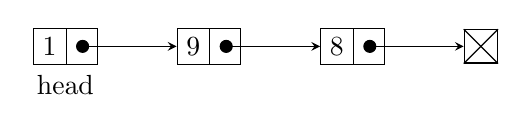
\begin{tikzpicture}[list/.style={rectangle split, rectangle split parts=2,
					draw, rectangle split horizontal}, >=stealth, start chain]

		\node[list,on chain] (A) {1};
		\node[list,on chain] (B) {9};
		\node[list,on chain] (C) {8};
		\node[on chain,draw,inner sep=6pt] (D) {};
		\draw (D.north east) -- (D.south west);
		\draw (D.north west) -- (D.south east);
		\draw[*->] let \p1 = (A.two), \p2 = (A.center) in (\x1,\y2) -- (B);
		\draw[*->] let \p1 = (B.two), \p2 = (B.center) in (\x1,\y2) -- (C);
		\draw[*->] let \p1 = (C.two), \p2 = (C.center) in (\x1,\y2) -- (D);

		\node[below=of A, yshift=1cm]{\alert{head}};
	\end{tikzpicture}

	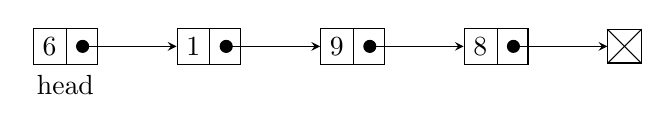
\begin{tikzpicture}[list/.style={rectangle split, rectangle split parts=2,
					draw, rectangle split horizontal}, >=stealth, start chain]

		\node[list,on chain] (A) {6};
		\node[list,on chain] (B) {1};
		\node[list,on chain] (C) {9};
		\node[list, on chain] (D) {8};
		\node[on chain,draw,inner sep=6pt] (E) {};
		\draw (E.north east) -- (E.south west);
		\draw (E.north west) -- (E.south east);
		\draw[*->] let \p1 = (A.two), \p2 = (A.center) in (\x1,\y2) -- (B);
		\draw[*->] let \p1 = (B.two), \p2 = (B.center) in (\x1,\y2) -- (C);
		\draw[*->] let \p1 = (C.two), \p2 = (C.center) in (\x1,\y2) -- (D);
		\draw[*->] let \p1 = (D.two), \p2 = (D.center) in (\x1,\y2) -- (E);

		\node[below=of A, yshift=1cm]{\alert{head}};
	\end{tikzpicture}

\end{frame}

\begin{frame}[fragile]

	\begin{columns}
		\column{.4\textwidth}<1->
		\begin{enumerate}
			\item Create a new node
			\item Set up the \alert{\texttt{next}}
			\item Update the \alert{\texttt{head}}
		\end{enumerate}
		\column{.6\textwidth}<2->
		{\large \faIcon{question-circle}}  \textbf{Question}: Can we even simplify the code using \texttt{Node}'s constructor?
	\end{columns}

	\scalebox{.85}{
		\begin{algorithm}[H]
			\caption{addFirst(head, element)}
			$x\gets Node(element)$ \\
			$x.next\gets head$ \\
			$head\gets x$
		\end{algorithm}
	}

\end{frame}

\begin{frame}[fragile]
	\frametitle{2.3 Common Operations: removeFirst()}
	To remove an element at the beginning in a list. The core idea is to \textbf{update the \alert{\texttt{head}} to the second node}.

	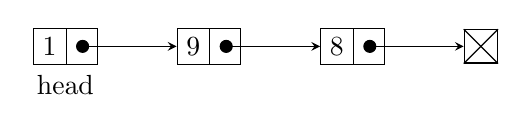
\begin{tikzpicture}[list/.style={rectangle split, rectangle split parts=2,
					draw, rectangle split horizontal}, >=stealth, start chain]

		\node[list,on chain] (A) {1};
		\node[list,on chain] (B) {9};
		\node[list,on chain] (C) {8};
		\node[on chain,draw,inner sep=6pt] (D) {};
		\draw (D.north east) -- (D.south west);
		\draw (D.north west) -- (D.south east);
		\draw[*->] let \p1 = (A.two), \p2 = (A.center) in (\x1,\y2) -- (B);
		\draw[*->] let \p1 = (B.two), \p2 = (B.center) in (\x1,\y2) -- (C);
		\draw[*->] let \p1 = (C.two), \p2 = (C.center) in (\x1,\y2) -- (D);

		\node[below=of A, yshift=1cm]{\alert{head}};
	\end{tikzpicture}

	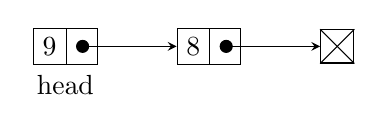
\begin{tikzpicture}[list/.style={rectangle split, rectangle split parts=2,
					draw, rectangle split horizontal}, >=stealth, start chain]

		\node[list,on chain] (A) {9};
		\node[list,on chain] (B) {8};
		\node[on chain,draw,inner sep=6pt] (D) {};
		\draw (D.north east) -- (D.south west);
		\draw (D.north west) -- (D.south east);
		\draw[*->] let \p1 = (A.two), \p2 = (A.center) in (\x1,\y2) -- (B);
		\draw[*->] let \p1 = (B.two), \p2 = (B.center) in (\x1,\y2) -- (D);

		\node[below=of A, yshift=1cm]{\alert{head}};
	\end{tikzpicture}

	\pause
	How do you think of it?
	\begin{minted}[bgcolor=LightGray, baselinestretch=1]{python}
head = head.next
    \end{minted}
\end{frame}


\begin{frame}

	\scalebox{.85}{
		\begin{algorithm}[H]
			\caption{removeFirst(head)}
			\If{isEmpty(head)} {
				raise an error
			} \Else {
				$head\gets head.next$
			}
		\end{algorithm}
	}

	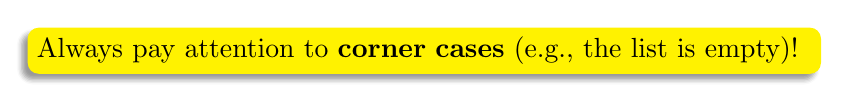
\begin{tikzpicture}
		\node[fill=yellow,blur shadow={shadow xshift=-0.5ex},
			text width=28em,anchor=south west,rounded corners]
		{Always pay attention to \textbf{corner cases} (e.g., the list is empty)!};
	\end{tikzpicture}

\end{frame}

\begin{frame}
	\frametitle{2.4 Common Operation: addLast()}

	To add an element at the end of the list. The core idea is to \textbf{set \alert{tail}'s \texttt{next} to the newly created node}.

	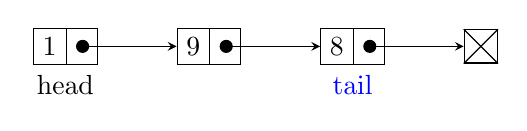
\begin{tikzpicture}[list/.style={rectangle split, rectangle split parts=2,
					draw, rectangle split horizontal}, >=stealth, start chain]

		\node[list,on chain] (A) {1};
		\node[list,on chain] (B) {9};
		\node[list,on chain] (C) {8};
		\node[on chain,draw,inner sep=6pt] (D) {};
		\draw (D.north east) -- (D.south west);
		\draw (D.north west) -- (D.south east);
		\draw[*->] let \p1 = (A.two), \p2 = (A.center) in (\x1,\y2) -- (B);
		\draw[*->] let \p1 = (B.two), \p2 = (B.center) in (\x1,\y2) -- (C);
		\draw[*->] let \p1 = (C.two), \p2 = (C.center) in (\x1,\y2) -- (D);

		\node[below=of A, yshift=1cm]{\alert{head}};

		\node[below=of C, yshift=1cm]{\textcolor{blue}{tail}};

	\end{tikzpicture}

	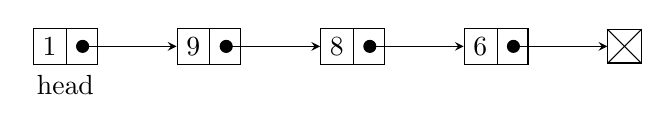
\begin{tikzpicture}[list/.style={rectangle split, rectangle split parts=2,
					draw, rectangle split horizontal}, >=stealth, start chain]

		\node[list,on chain] (A) {1};
		\node[list,on chain] (B) {9};
		\node[list,on chain] (C) {8};
		\node[list, on chain] (E) {6};
		\node[on chain,draw,inner sep=6pt] (D) {};
		\draw (D.north east) -- (D.south west);
		\draw (D.north west) -- (D.south east);
		\draw[*->] let \p1 = (A.two), \p2 = (A.center) in (\x1,\y2) -- (B);
		\draw[*->] let \p1 = (B.two), \p2 = (B.center) in (\x1,\y2) -- (C);
		\draw[*->] let \p1 = (C.two), \p2 = (C.center) in (\x1,\y2) -- (E);

		\draw[*->] let \p1 = (E.two), \p2 = (E.center) in (\x1,\y2) -- (D);

		\node[below=of A, yshift=1cm]{\alert{head}};

	\end{tikzpicture}
\end{frame}

\begin{frame}

	\begin{columns}
		\column{.4\textwidth}
		\begin{enumerate}
			\item Locate the \alert{tail}
			\item Create a new node
			\item Set up \alert{tail}'s \texttt{next}
		\end{enumerate}
		\column{.6\textwidth}
		{\large \faIcon{question-circle}}  \textbf{Question}: How to locate the \alert{\texttt{tail}}?
	\end{columns}

	\pause
	\scalebox{.85}{
		\begin{algorithm}[H]
			\caption{addLast(head, element)}
			$tail\gets head$ \\
			\While{tail.next $\neq$ null} {
				$tail\gets tail.next$
			}
			$tail.next\gets Node(element)$
		\end{algorithm}
	}

	{\large \faIcon{lightbulb}} \textbf{Think twice}: Does the code work when the list is empty?

\end{frame}

\begin{frame}
	\scalebox{.85}{
		\begin{algorithm}[H]
			\caption{addLast(head, element)}
			\If {isEmpty(head)} {
				$head\gets Node(element)$
			}
			\Else {
				$tail\gets head$ \\
				\While{tail.next $\neq$ null}{
					$tail\gets tail.next$
				}
				$tail.next\gets Node(element)$
			}
		\end{algorithm}
	}

	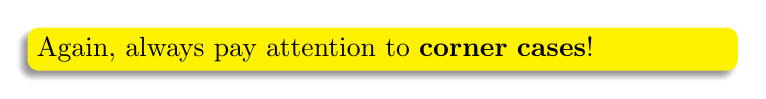
\begin{tikzpicture}
		\node[fill=yellow,blur shadow={shadow xshift=-0.5ex},
			text width=25em,anchor=south west,rounded corners]
		{Again, always pay attention to \textbf{corner cases}!};
	\end{tikzpicture}
\end{frame}

\begin{frame}
	\frametitle{Revisit tail}

	\begin{columns}
		\column{.4\textwidth}
		\begin{enumerate}
			\item Locate the \alert{tail}
			\item Create a new node
			\item Set up \alert{tail}'s \texttt{next}
		\end{enumerate}
		\column{.6\textwidth}
		{\large \faIcon{question-circle}} \textbf{Question}: What is the time complexity of \texttt{addLast()}?
	\end{columns}

	\pause
	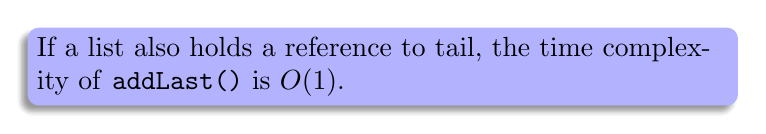
\begin{tikzpicture}
		\node[fill=blue!30,blur shadow={shadow xshift=-0.5ex},
			text width=25em,anchor=south west,rounded corners]
		{If a list also holds a reference to \alert{tail}, the time complexity of \texttt{addLast()} is $O(1)$.};
	\end{tikzpicture}

	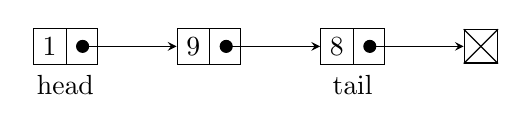
\begin{tikzpicture}[list/.style={rectangle split, rectangle split parts=2,
					draw, rectangle split horizontal}, >=stealth, start chain]

		\node[list,on chain] (A) {1};
		\node[list,on chain] (B) {9};
		\node[list,on chain] (C) {8};
		\node[on chain,draw,inner sep=6pt] (D) {};
		\draw (D.north east) -- (D.south west);
		\draw (D.north west) -- (D.south east);
		\draw[*->] let \p1 = (A.two), \p2 = (A.center) in (\x1,\y2) -- (B);
		\draw[*->] let \p1 = (B.two), \p2 = (B.center) in (\x1,\y2) -- (C);
		\draw[*->] let \p1 = (C.two), \p2 = (C.center) in (\x1,\y2) -- (D);

		\node[below=of A, yshift=1cm]{\alert{head}};

		\node[below=of C, yshift=1cm]{\alert{tail}};

	\end{tikzpicture}

	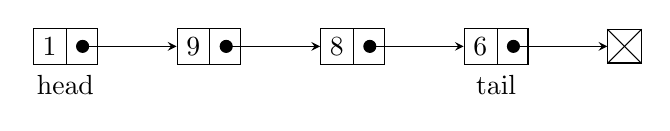
\begin{tikzpicture}[list/.style={rectangle split, rectangle split parts=2,
					draw, rectangle split horizontal}, >=stealth, start chain]

		\node[list,on chain] (A) {1};
		\node[list,on chain] (B) {9};
		\node[list,on chain] (C) {8};
		\node[list, on chain] (E) {6};
		\node[on chain,draw,inner sep=6pt] (D) {};
		\draw (D.north east) -- (D.south west);
		\draw (D.north west) -- (D.south east);
		\draw[*->] let \p1 = (A.two), \p2 = (A.center) in (\x1,\y2) -- (B);
		\draw[*->] let \p1 = (B.two), \p2 = (B.center) in (\x1,\y2) -- (C);
		\draw[*->] let \p1 = (C.two), \p2 = (C.center) in (\x1,\y2) -- (E);

		\draw[*->] let \p1 = (E.two), \p2 = (E.center) in (\x1,\y2) -- (D);

		\node[below=of A, yshift=1cm]{\alert{head}};
		\node[below= of E, yshift=1cm]{\alert{tail}};
	\end{tikzpicture}

\end{frame}

\begin{frame}[fragile]
	\frametitle{Task}

	\begin{block}{Linked Lists}
		Many implementations for linked lists would hold three fields: \texttt{head}, \texttt{tail}, and \texttt{size}.
	\end{block}

	{\large \faIcon{book-reader}} Please read \href{https://chenzhongpu.github.io/data-structure-swufe/list/linkedlist.html#addlast-add-an-element-at-the-end}{addLast(): add an element at the end} in Section 3.3.1 to understand the pseudo-code of \texttt{addLast(head, tail, element)};

\end{frame}

\begin{frame}
	\frametitle{2.5 Common Operations: removeLast()}

	\begin{columns}
		\column{.45\textwidth}<1->

		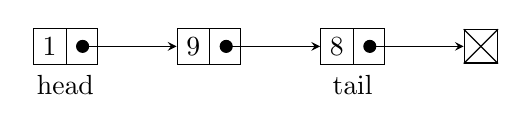
\begin{tikzpicture}[list/.style={rectangle split, rectangle split parts=2,
						draw, rectangle split horizontal}, >=stealth, start chain]

			\node[list,on chain] (A) {1};
			\node[list,on chain] (B) {9};
			\node[list,on chain] (C) {8};
			\node[on chain,draw,inner sep=6pt] (D) {};
			\draw (D.north east) -- (D.south west);
			\draw (D.north west) -- (D.south east);
			\draw[*->] let \p1 = (A.two), \p2 = (A.center) in (\x1,\y2) -- (B);
			\draw[*->] let \p1 = (B.two), \p2 = (B.center) in (\x1,\y2) -- (C);
			\draw[*->] let \p1 = (C.two), \p2 = (C.center) in (\x1,\y2) -- (D);

			\node[below=of A, yshift=1cm]{\alert{head}};
			\node[below=of C, yshift=1cm]{\alert{tail}};

		\end{tikzpicture}

		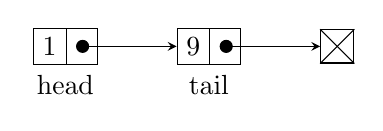
\begin{tikzpicture}[list/.style={rectangle split, rectangle split parts=2,
						draw, rectangle split horizontal}, >=stealth, start chain]

			\node[list,on chain] (A) {1};
			\node[list,on chain] (B) {9};
			\node[on chain,draw,inner sep=6pt] (D) {};
			\draw (D.north east) -- (D.south west);
			\draw (D.north west) -- (D.south east);
			\draw[*->] let \p1 = (A.two), \p2 = (A.center) in (\x1,\y2) -- (B);
			\draw[*->] let \p1 = (B.two), \p2 = (B.center) in (\x1,\y2) -- (D);

			\node[below=of A, yshift=1cm]{\alert{head}};
			\node[below=of B, yshift=1cm]{\alert{tail}};

		\end{tikzpicture}
		\column{.55\textwidth}<2->
		\begin{enumerate}
			\item Locate the second node to last $x$
			\item Update $x$'s \texttt{next}
			\item Update \texttt{tail}
		\end{enumerate}
	\end{columns}

	To remove an element at the end of a list. The core idea is to \textbf{update the tail to the second node to last}.

\end{frame}

\begin{frame}

	\scalebox{.85}{
		\begin{algorithm}[H]
			\caption{removeLast(head, tail)}
			$x\gets head$ \\
			\While{x.next $\neq$ tail} {
				$x\gets x.next$
			}
			$x.next\gets null$ \\
			$tail\gets x$
		\end{algorithm}
	}

	{\large \faIcon{lightbulb}} \textbf{Think twice}: Does the code work when the list is empty or the size is 1?

\end{frame}

\begin{frame}

	\scalebox{.82}{
		\begin{algorithm}[H]
			\setstretch{.9}
			\caption{removeLast(head, tail)}
			\If{isEmpty(head)} {
				\tcp{case 1: it is empty}
				raise an error
			}\ElseIf{head == tail} {
				\tcp{case 2: the size is 1}
				$head\gets null$ \\
				$tail\gets null$
			}\Else{
				\tcp{case 3: the size is greater than 1}
				$x\gets head$ \\
				\While{x.next $\neq$ tail}{
					$x\gets x.next$
				}
				$x.next\gets null$ \\
				$tail\gets x$
			}
		\end{algorithm}
	}

\end{frame}

\begin{frame}[fragile]
	\frametitle{removeLast(): tail is not stored}
	Try to implement the algorithm \alert{removeLast(head)}.
\end{frame}

{\setbeamercolor{palette primary}{fg=black, bg=yellow}
\begin{frame}[standout]
	Try to implement those common operations in Python or Java based on the pseudo-code after class.
\end{frame}
}

\begin{frame}
	\section{\textcolor{darkmidnightblue}{3. Stacks And Queues}}
	How to implement stacks and queues based on linked lists?
\end{frame}

\begin{frame}
	\frametitle{3.1 Stacks}
	To follow the \textbf{LIFO} policy, elements should be pushed and popped from the same end.
	\begin{columns}
		\column{.54\textwidth}
		\begin{table}
			\begin{tabular}{ll}
				\toprule
				Operation              & Time Complexity \\
				\midrule
				\texttt{addFirst()}    & $O(1)$          \\
				\texttt{addLast()}     & $O(1)$          \\
				\texttt{removeFirst()} & $O(1)$          \\
				\texttt{removeLast()}  & $O(N)$          \\
				\bottomrule
			\end{tabular}
		\end{table}
		\column{.45\textwidth}
		{\large \faIcon{question-circle}} \textbf{Question}: As for stacks, which end is better (\texttt{head} or \texttt{tail})?
	\end{columns}

\end{frame}

\begin{frame}
	\frametitle{3.2 Queues}
	To follow the \textbf{FIFO} policy, elements should be enqueued and dequeued from the different end.

	\begin{itemize}
		\item \texttt{enqueue()}: \texttt{addLast()} in a linked list
		\item \texttt{dequeue()}: \texttt{removeFirst()} in a linked list
	\end{itemize}

\end{frame}

\begin{frame}
	\section{\textcolor{darkmidnightblue}{4. More Operations}}
	Operations apart from \texttt{addFirst()/addLast()/removeFirst()/removeLast()}
\end{frame}

\begin{frame}
	\frametitle{4.1 get(i)}
	To return the i-th node of a list.

	\scalebox{.8}{
		\begin{algorithm}[H]
			\caption{get(i)}
			\If{i > size - 1 or i < 0} {
				raise OutOfTheBound error
			}
			$cnt\gets 0$ \\
			$x\gets head$ \\
			\While{cnt < i}{
				$x\gets x.next$ \\
				$cnt\gets cnt + 1$
			}
			\Return{x}
		\end{algorithm}
	}

\end{frame}

\begin{frame}
	\frametitle{Exercise}
	{\large \faIcon{code}} Please write the pseudo-code of \texttt{indexOf(k)} for a linked list.

\end{frame}

\begin{frame}
	\frametitle{4.2 set(i, k)}
	To set the item of the i-th node of a list to $k$.

	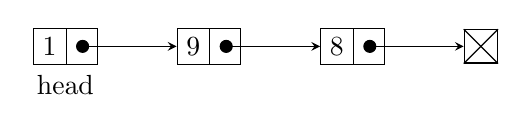
\begin{tikzpicture}[list/.style={rectangle split, rectangle split parts=2,
					draw, rectangle split horizontal}, >=stealth, start chain]

		\node[list,on chain] (A) {1};
		\node[list,on chain] (B) {9};
		\node[list,on chain] (C) {8};
		\node[on chain,draw,inner sep=6pt] (D) {};
		\draw (D.north east) -- (D.south west);
		\draw (D.north west) -- (D.south east);
		\draw[*->] let \p1 = (A.two), \p2 = (A.center) in (\x1,\y2) -- (B);
		\draw[*->] let \p1 = (B.two), \p2 = (B.center) in (\x1,\y2) -- (C);
		\draw[*->] let \p1 = (C.two), \p2 = (C.center) in (\x1,\y2) -- (D);

		\node[below=of A, yshift=1cm]{\alert{head}};
	\end{tikzpicture}

	\pause
	\scalebox{.85}{
		\begin{algorithm}[H]
			\caption{set(i, k)}
			$x\gets get(i)$ \\
			$x.item\gets k$
		\end{algorithm}
	}

\end{frame}

\begin{frame}
	\frametitle{4.3 insert(i, k)}
	To insert a node whose item is $k$ at position $i$.

	\scalebox{.8}{
		\begin{algorithm}[H]
			\caption{insert(i, k)}
			\If{i == 0} {
				addFirst(k)
			}\ElseIf{i == size} {
				addLast(k)
			}\Else {
				$x\gets get(i - 1)$ \\
				$x.next\gets Node(k, x.next)$
			}
		\end{algorithm}
	}

\end{frame}

\begin{frame}
	\frametitle{Exercise}
	{\large \faIcon{code}} Please write the pseudo-code of \texttt{delete(i)} for a linked list.
\end{frame}

\begin{frame}

	\section{\textcolor{darkmidnightblue}{Conclusion}}
	\begin{enumerate}
		\item ADT
		\item Array List vs. Linked List
		\item Adding and removing elements on a linked list
	\end{enumerate}
\end{frame}

\end{document}
